\documentclass[12pt,a4paper]{article}
\usepackage[spanish,es-tabla]{babel}
\usepackage{float}							% Insertar figuras


\usepackage[utf8]{inputenc} % Escribir con acentos, ~n...
\usepackage{eurosym} % s´ımbolo del euro
\newcommand{\horrule}[1]{\rule{\linewidth}{#1}} % Create horizontal rule command with 1 argument of height
\usepackage{listings}             % Incluye el paquete listing
\usepackage{amsfonts}
\usepackage{booktabs}
\usepackage{subfig}

\usepackage[cache=false]{minted}
\usepackage{graphics,graphicx, float} %para incluir imágenes y colocarlas
\usepackage{hyperref}
\hypersetup{
	colorlinks,
	citecolor=black,
	filecolor=black,
	linkcolor=black,
	urlcolor=black
}
\usepackage{multirow}
\usepackage{array}
\usepackage{diagbox}
\usepackage{listings}

\lstset{language=Java,
	keywordstyle=\color{RoyalBlue},
	basicstyle=\scriptsize\ttfamily,
	commentstyle=\ttfamily\itshape\color{gray},
	stringstyle=\ttfamily,
	showstringspaces=false,
	breaklines=true,
	frameround=ffff,
	frame=single,
	rulecolor=\color{black}}
\title{
\normalfont \normalsize 
\textsc{{\bf Simulación de Sistemas (2019-2020)} \\ Grado en Ingeniería Informática \\ Universidad de Granada} \\ [25pt] % Your university, school and/or department name(s)
\horrule{0.5pt} \\[0.4cm] % Thin top horizontal rule
\huge Práctica 2 \\ % The assignment title
\horrule{2pt} \\[0.5cm] % Thick bottom horizontal rule

\includegraphics{images/logo.png}	
}

\author{Antonio Jesús Heredia Castillo} % Nombre y apellidos

\date{\normalsize\today} % Incluye la fecha actual

%----------------------------------------------------------------------------------------
% DOCUMENTO
%----------------------------------------------------------------------------------------

\begin{document}

\maketitle % Muestra el Título

\newpage
\tableofcontents % para generar el índice de contenidos
\newpage %inserta un salto de página
\listoffigures
\newpage
\section{Mi Segundo Modelo de Simulación de Monte Carlo}
\subsection{Modelización por Monte Carlo}
Para probar los resultados practicos de la modelización por Monte Carlo he realizado una serie de experimentos con distintos valores (los especificados en el guión de la practica). Estos valores será:
\begin{enumerate}
	\item Ganancia: 10 Perdida: 1
	\item Ganancia: 10 Perdida: 5
	\item Ganancia: 10 Perdida:10
\end{enumerate}
Para ver como afecta la simulación de mas o menos días, los experimentos anteriores los simularemos con 100,1000,5000,10000 y 100000 días. Al usar números aleatorios podemos presuponer que cuantas mas días simulemos tendremos una visión mas clara de lo que podrá ocurrir. \\ En la siguiente tabla podemos ver los datos generados usando una distribución uniforme. 
\begin{table}[H]
\begin{tabular}{ccccc} \toprule
	{Ganancia} & {Perdida} & {Repeticiones} & {Mejor pedido} & {Mejor ganancia} \\ \midrule
	10  & 1 & 100 & 100 & 483.769989 \\
	10  & 1 & 1000 & 77 & 460.899994 \\
	10  & 1 & 5000 & 90 & 453.419800 \\
	10  & 1 & 10000 & 89 & 453.176788 \\
	10  & 1 & 100000 & 89 & 450.824799 \\ \midrule
	
	10  & 5 & 100 & 68 & 373.850006 \\
	10  & 5 & 1000 & 69 & 345.690002 \\
	10  & 5 & 5000 & 61 & 335.872009 \\
	10  & 5 & 10000 & 67 & 332.891510 \\
	10  & 5 & 100000 & 70 & 330.063629 \\ \midrule
	
	10  & 10 & 100 & 61 & 292.399994 \\
	10  & 10 & 1000 & 51 & 249.539993 \\
	10  & 10 & 5000 & 57 & 249.584000 \\
	10  & 10 & 10000 & 54 & 251.475998 \\
	10  & 10 & 100000 & 47 & 247.018402\\ \midrule	
\end{tabular}
\caption{Usando el generador de datos a} \label{tab:genDataA}
\end{table}
En los datos recogidos en las distintas tablas podremos comparar el funcionamiento de los distintos generadores de datos. Una cosa que va a ser común en todos los generadores sera que a medida que haces mas simulaciones los precios son mas bajos. Esto tiene una sencilla explicación, y es que con pocas simulaciones podemos tener una en que de la casualidad que todos los días vence todos los periódicos pero en cambio, al realizar un numero suficiente de simulaciones tenemos que las media de periódicos vendidos se vuelve parecida. \\ En esta tabla podemos ver los datos obtenidos en una distribución proporcional. 
\begin{table}[H]
	\begin{tabular}{ccccc} \toprule
		{Ganancia} & {Perdida} & {Repeticiones} & {Mejor pedido} & {Mejor ganancia} \\ \midrule
		10  & 1 & 100 & 84 & 351.380005 \\
		10  & 1 & 1000 & 74 & 304.058990 \\
		10  & 1 & 5000 & 74 & 286.687805 \\
		10  & 1 & 10000 & 76 & 288.766602 \\
		10  & 1 & 100000 & 73 & 284.473694 \\ \midrule
		
		10  & 5 & 100 & 39 & 227.850006 \\
		10  & 5 & 1000 & 48 & 203.309998 \\
		10  & 5 & 5000 & 49 & 192.845001\\
		10  & 5 & 10000 & 44 & 191.050995\\
		10  & 5 & 100000 & 41 & 188.323486 \\ \midrule
		
		10  & 10 & 100 & 32 & 178.600006 \\
		10  & 10 & 1000 & 34 & 148.220001 \\
		10  & 10 & 5000 & 29 & 139.632004 \\
		10  & 10 & 10000 & 28 & 136.710007 \\
		10  & 10 & 100000 & 31 & 134.704605\\ \midrule	
	\end{tabular}
	\caption{Usando el generador de datos b} \label{tab:genDataB}
\end{table}
Sin duda la distribución proporcional es la que peores datos nos devuelve. \\
En la siguiente tabla podemos ver los datos obtenidos a partir de la distribución triangular.
\begin{table}[H]
	\begin{tabular}{ccccc} \toprule
		{Ganancia} & {Perdida} & {Repeticiones} & {Mejor pedido} & {Mejor ganancia} \\ \midrule
		10  & 1 & 100 & 73 & 529.580017 \\
		10  & 1 & 1000 & 79 & 476.423004
		 \\
		10  & 1 & 5000 & 75 & 470.261200 \\
		10  & 1 & 10000 & 77 & 465.843414 \\
		10  & 1 & 100000 & 80 & 465.232147 \\ \midrule
		
		10  & 5 & 100 & 68 & 438.200012 \\
		10  & 5 & 1000 & 62 & 407.975006 \\
		10  & 5 & 5000 & 56 & 388.279999 \\
		10  & 5 & 10000 & 60 & 389.065491 \\
		10  & 5 & 100000 & 59 & 386.263916		 \\ \midrule
		
		10  & 10 & 100 & 61 & 382.000000
		 \\
		10  & 10 & 1000 & 53 & 342.059998 \\
		10  & 10 & 5000 & 48 & 338.799988 \\
		10  & 10 & 10000 & 51 & 337.914001 \\
		10  & 10 & 100000 & 50 & 334.353210\\ \midrule	
	\end{tabular}
	\caption{Usando el generador de datos c} \label{tab:genDataC}
\end{table}
Como se puede observar en la Figura \ref{f:compgeneradoresBueno}, sin duda el mejor resultado lo obtenemos usando la distribución triangular. Esto puede ocurrir por un motivo y es que la distribución y triangular favorece los datos que se encuentran en el centro y esto puede ser una buena estrategia ya que no va vender ni muchos ni pocos periódicos, haciendo así que las perdidas no suban demasiado respecto a las ventas.

\begin{figure}[H]
	\centering
	\subfloat[100000 simulaciones]{
		\label{f:compgeneradoresBueno}
		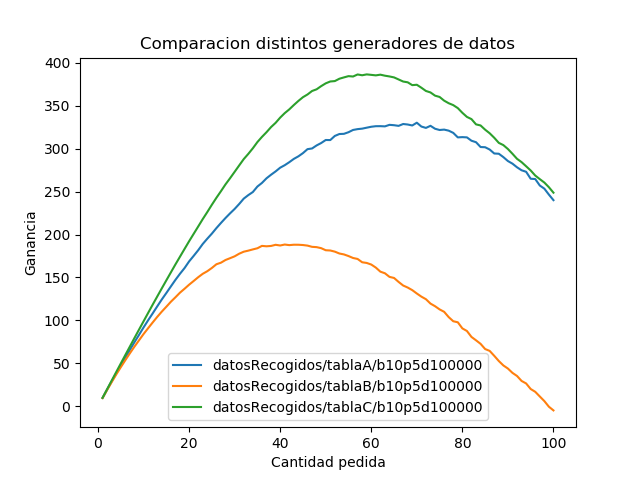
\includegraphics[width=0.5\textwidth]{images/compGeneradores}}
	\subfloat[100 simulaciones]{
		\label{f:compgeneradoresMalo}
		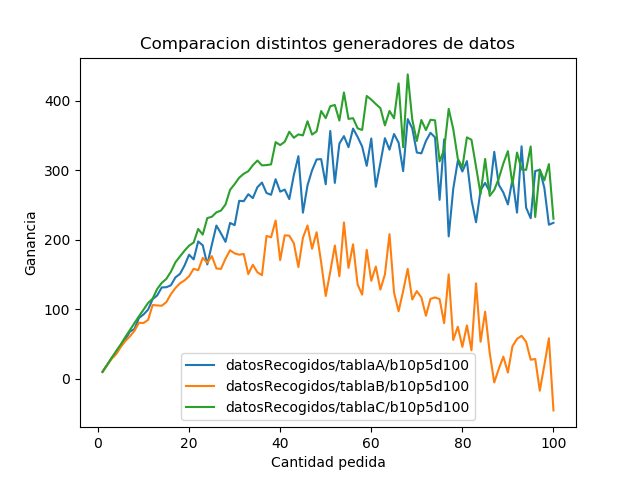
\includegraphics[width=0.5\textwidth]{images/compGeneradoresMal.png}}
	\caption{Diferencias entre la cantidad de simulaciones.}
	\label{f:compgeneradores}
\end{figure}

Otra cosa interesante que podemos analizar en la Figura \ref{f:compgeneradores} es como armoniza los resultados con muchas simulaciones. Esto se debe a que con pocas simulaciones podemos tener datos muy  buenos o muy malos ya que depende mucho de los datos que se generen. 
\begin{figure}[H]
	\centering
	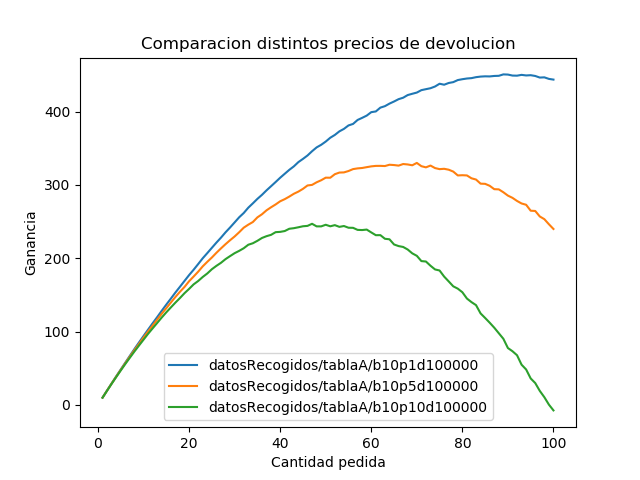
\includegraphics[width=0.7\linewidth]{images/compCosteDevolucionpng}
	\caption{Diferencias entre los costes de devolución}
	\label{fig:compcostedevolucionpng}
\end{figure}
Aunque era de esperar podemos ver en la Figura \ref{fig:compcostedevolucionpng} como cuanto mas nos cueste devolver un periódico mas recomendable es pedir de forma controlada. Ya que si podimos muchos pero no los vendemos podemos llegar a tener perdidas. 
\subsection{Modificaciones del Modelo}
Para esta parte de la practica vamos a trabajar sobre el modelo de Monte Carlo anterior pero añadiéndole algunas mejoras. 
\subsubsection{Coste de devolución fijo}
La base del modelo sera el anterior pero esta vez en vez de pagar según la cantidad de periódicos que devuelvas la devolución tendrá un coste fijo. Veremos como influye esto a la hora de ver las ganancias que tendremos. \\ Esta vez las variables serán:
\begin{enumerate}
	\item Ganancia: 10 Coste devolución: 10
	\item Ganancia: 10 Coste devolución: 50
	\item Ganancia: 10 Coste devolución:100
\end{enumerate}
Y como hemos visto que cuantas mas ejecuciones mas preciso sera el modelo, lo ejecutaremos 100000 veces.
\begin{table}[H]
	\begin{tabular}{ccccc} \toprule
		{Repeticiones} & {Ganancia} & {Perdida} &  {Mejor pedido} & {Mejor ganancia} \\ \midrule
		a &10  & 10 & 96 & 486.497528 \\
		a &10  & 50  & 94 & 447.436249\\
		a &10  & 100 & 92 & 400.943359 \\
		\midrule
		b &10  & 10 & 98 & 321.195709 \\
		b &10  & 50 & 97 & 281.260712 \\
		b &10  & 100 & 76 & 231.906296 \\  
		\midrule
		c &10  & 10& 94 & 490.859680\\
		c &10  & 50& 91 & 451.618713 \\
		c &10  & 100& 77 & 403.607269 \\
		\midrule	
	\end{tabular}
	\caption{Modificación 1} \label{tab:mod1}
\end{table}
Como podemos ver en la Tabla \ref{tab:mod1}, al igual que pasaba antes el generador de tipo triangular nos da las mejores ganancias.  Aunque aqui lo que podemos ver es como no influye tanto los costes fijos a la hora de tener el mejor pedido. Ya que nos importa poco cuantos devolvamos que siempre vamos a tener que pagar lo mismo. Esto se puede ver en la diferencia entre las mejores ganancias, que entre cada una los separa lo mismo que en los costes fijos por devolución. 
\begin{figure}[H]
	\centering
	\subfloat[Tabla A]{
		\label{f:modTablaA}
		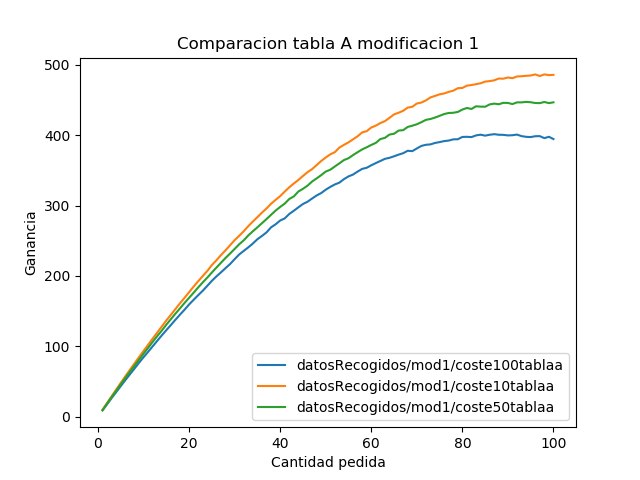
\includegraphics[width=0.5\textwidth]{images/mod1TablaA.png}}
	\subfloat[Tabla B]{
		\label{f:modTablaB}
		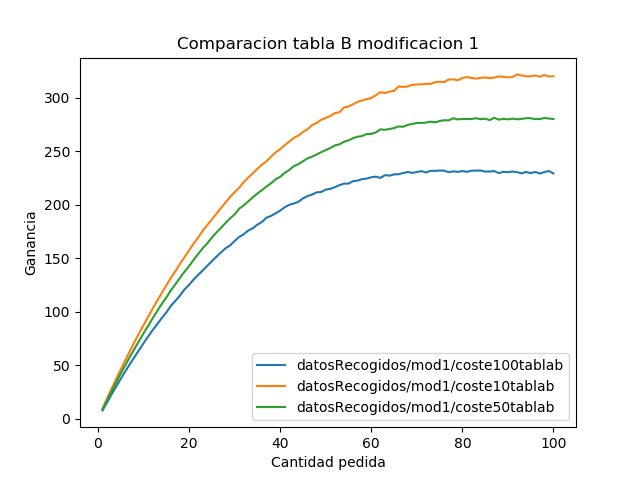
\includegraphics[width=0.5\textwidth]{images/mod1TablaB.png}}
		\caption{Ganancias con coste fijos.}
		\subfloat[Tabla C]{
		\label{f:modTablaC}
		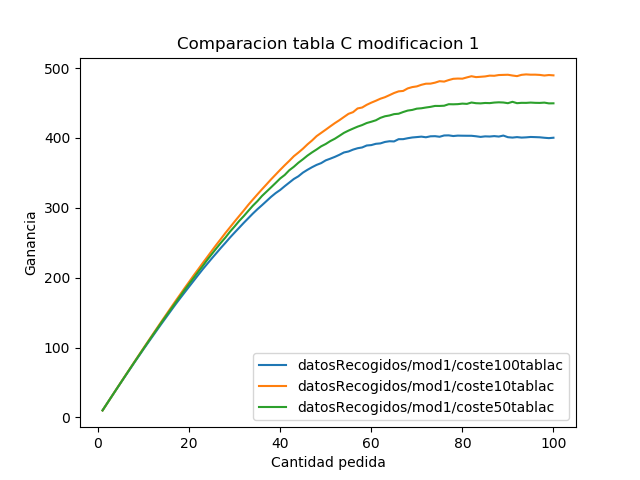
\includegraphics[width=0.5\textwidth]{images/mod1TablaC.png}}
	\caption{Ganancias con coste fijos.}
	\label{f:mod1}
\end{figure}
Como podemos ver en la Figura \ref{f:mod1} todas las tablas se comportan de la misma manera. Una vez llegan a una cantidad de pedidos, se comportan casi de forma constante y no crecen ni disminuyen los beneficios. 
\subsubsection{Coste de devolución fijo pero decidiendo si devolver o no}
En esta modificación añadimos otra mejora. Esta vez ademas de tener un coste fijo de devolución el kioskero podra decidir cuando devolver o no, teniendo en cuenta cuanto perdería por periódico en caso de que no lo hiciera. Para realizar la comparación fijaremos tanto la cantidad de simulaciones como la ganancia y el coste de devolución.
Este ejemplo lo ejecutaremos con las siguiente variables:
\begin{enumerate}
	\item Ganancia: 10 Coste devolución: 100 Coste no devolución: 5
	\item Ganancia: 10 Coste devolución: 100 Coste no devolución: 10
	\item Ganancia: 10 Coste devolución: 100 Coste no devolución: 15
\end{enumerate}
\begin{table}[H]
	\begin{tabular}{cccccc} \toprule
		{Repeticiones} & {Ganancia} & {Coste fijo}&{Perdida} &  {Mejor pedido} & {Mejor ganancia} \\ \midrule
		a &10  & 10 & 5 &88 & 411.015045 \\
		a &10  & 50  & 10 &92 &406.135590\\
		a &10  & 100 &15 & 90 & 404.093689 \\
		\midrule
		b &10  & 10 & 5 &72 & 238.302399 \\
		b &10  & 50 & 10 &71 & 234.886505 \\
		b &10  & 100 & 15 &77 & 233.997498 \\  
		\midrule
		c &10  & 10&5 & 71 & 416.182068\\
		c &10  & 50&10 & 73 & 408.292480 \\
		c &10  & 100&15 & 77 & 406.603485\\
		\midrule	
	\end{tabular}
	\caption{Modificación 2} \label{tab:mod2}
\end{table}
Como esta vez hemos fijado los costes fijos y lo que variamos son las perdidas por no devolver lo que tenemos es que como solo devuelve cuando esta seguro de que las perdidas van a ser mayores que los costes fijos no nos importa el valor de los mismo. De esta forma podríamos aprovechar al máximo las ganancias. A diferencia que en la Figura \ref{f:mod1} en la Figura \ref{f:mod2} podemos ver es que aquí si importa que pidamos periódicos de mas ya que no se comporta de manera constante. Si pedimos de mas los beneficios empiezan a bajar de forma muy suave. 
\begin{figure}[H]
	\centering
	\subfloat[Tabla A]{
		\label{f:mod2TablaA}
		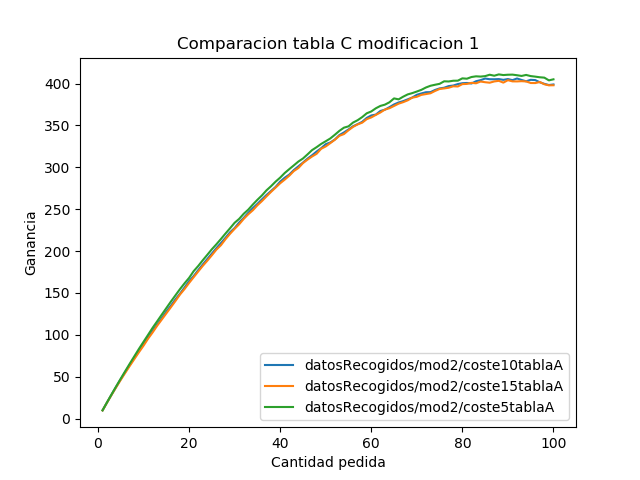
\includegraphics[width=0.5\textwidth]{images/mod2TablaA.png}}
	\subfloat[Tabla B]{
		\label{f:mod2TablaB}
		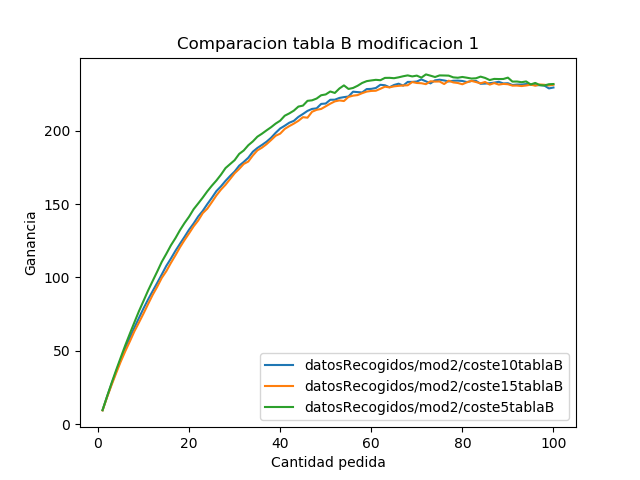
\includegraphics[width=0.5\textwidth]{images/mod2TablaB.png}}
	\caption{Ganancias con costes fijos decidiendo si devolver o no.}
	\subfloat[Tabla C]{
		\label{f:mod2TablaC}
		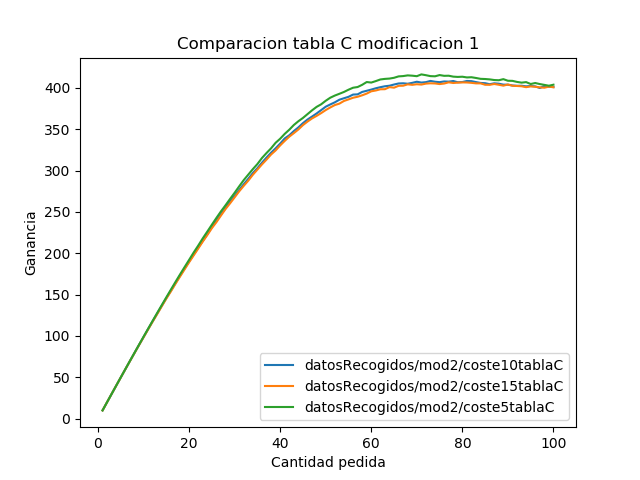
\includegraphics[width=0.5\textwidth]{images/mod2TablaC.png}}
	\caption{Ganancias con costes fijos decidiendo si devolver o no.}
	\label{f:mod2}
\end{figure}
\section{Generadores de datos}
\subsection{Mejorando los Generadores}
Para mejorar las tablas vamos a usar varios métodos para cambiar la forma en que se generan.
\subsubsection{Reordenar valores}
En este caso solo tenemos que modificar el generador C, es decir el de distribución triangular. Esto se debe a que en el a los valores están ordenados puesto que son iguales en cambio y en el b si que se generan de forma decreciente. Para ello hemos modificado el generador que nos daba el profesor para generarlo de forma decreciente sin tener que re ordenarlos después. Ademas he tenido que hacer cambios tanto en la generación de los otros dos metodos como en la función que nos devuelve un valor puesto que he usado unos pares de valores para guardar tanto el valor como su probabilidad acomulada ya que esta vez el indice donde se encuentra no corresponde con el valor que es. \\ Para ver una comparativa de como es de eficiente cada uno los ejecutare varias veces para comprobar tiempos.
\subsubsection{Busqueda binaria}
En este método la generación de las tablas no cambia, lo que cambiaremos es usar una búsqueda binaria a la hora de obtener un valor. Haciendo así una búsqueda mas rápida que nos puede venir mejor. 
\subsubsection{Generación en tiempo constante}
Para este metodo no usaremos una tabla, simplemente generaremos un dato a partir de lo devuelto por la funcion $uniforme()$ multiplicandolo por el valor maximo que queremos obtener. Esto funciona gracias a que lo que nos devuelve $uniforme()$ se encuentra entre 0 y 1.
\subsubsection{Comparación de los distintos metodos.}
Para la comparación como en el generador 3 siempre se da los mismos datos, he usado los mismos datos recogidos para las tres comparaciones. 


Como podemos ver en la Figura \ref{fig:tablaA} el original como su modificación para el generador 1 son casi iguales. La pequeña diferencia que existe es por el hecho de trabajar con pares de valores. En cambio en el la obtención de datos usando busqueda binaria si que vemos una gran mejora. El tiempo de ejecución se disminuye hasta la mitad, haciendo así una buena optimización para cuando tengamos que ejecutarlo muchas veces. Aunque sin dudarlo el que mejor funciona en este caso y en los siguientes es el generador en tiempo constante que por mucho que aumentemos las ejecuciones apenas aumenta el tiempo de ejecución. Por tanto el generador en tiempo constante siempre va a ser el mas rápido. 
\begin{figure}[H]
	\centering
	\subfloat[Tabla A]{
	\label{fig:tablaA}
		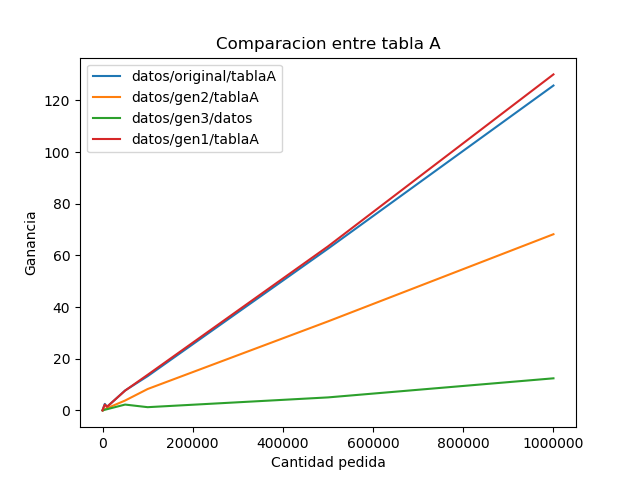
\includegraphics[width=0.5\textwidth]{images/genTablaA.png}}
	\subfloat[Tabla B]{
		\label{f:tablaB}
		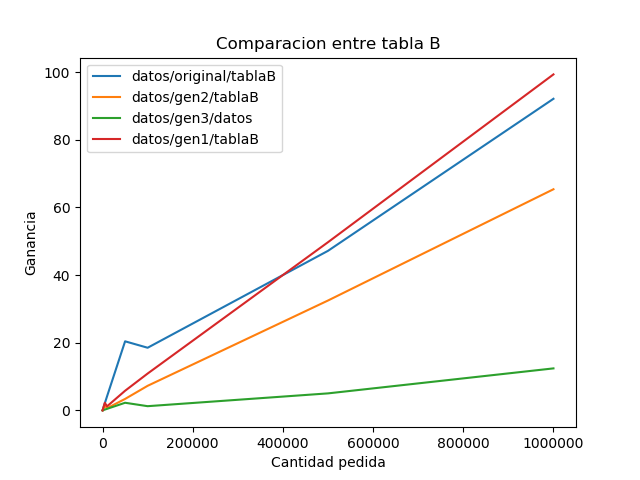
\includegraphics[width=0.5\textwidth]{images/genTablaB.png}}
	\caption{Diferencias de tiempo entre las distintas mejoras.}
	\subfloat[Tabla C]{
		\label{f:tablaC}
		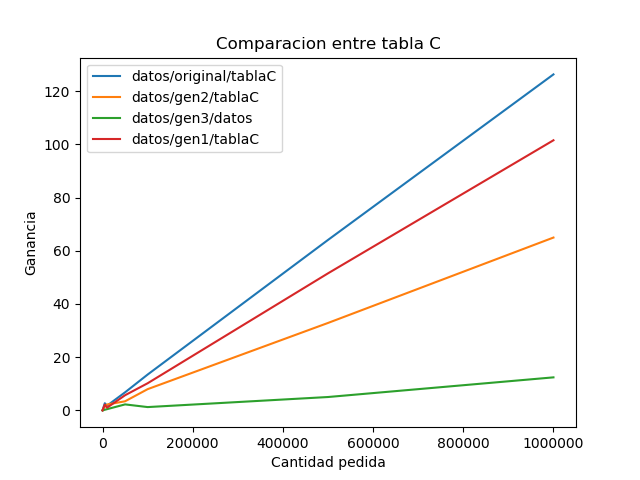
\includegraphics[width=0.5\textwidth]{images/genTablaC.png}}
	\caption{Diferencias de tiempo entre las distintas mejoras.}
	\label{f:generadores1}
\end{figure}
Al general la tabla con los datos de forma decreciente en la distribución triangular vamos a notar una gran mejora respecto a generarla de forma normal (Figura \ref{f:tablaC}). Aunque sigue siempre mas lento que si usáramos la búsqueda binaria que funciona de forma muy rápida. \\ \\Por lo tanto si tuviéramos que elegir algún método yo usaría la mejora de usar la búsqueda binaria. Por que nos permite tener distintas distribuciones pero sin gastar excesivo tiempo a la hora de generar los datos. La generación en tiempo constante aunque es muy rápida nos impide usar distintas distribuciones por lo tanto no seria una opción adecuada para segun que tiempo de modelo de Monte Carlo. 
\subsection{Generadores congruenciales}
En esta sección veremos como funciona los generadores de datos aleatorios congruenciales. Para ello haremos pruebas con diferentes generadores ademas de usar dos $a$ diferentes. Esto lo hacemos para ver como afecta las distintas variables a los generadores y como el efecto de la semilla. 
\begin{itemize}
	\item $a_1=2061$
	\item $a_2=2060$
\end{itemize}
En todos los generadores y pruebas fijaremos semilla inicial a $x=19$, para que esto no influya a la hora de generar.
\begin{table}[H]
	\begin{tabular}{cccc} \toprule
		{Tipo Generador} & {a} & {Semilla}& {Ciclos} \\ \midrule
		Usando \% & 2061  & 19 & 1000 \\
		Usando \% & 2060  & 19  & 4\\
		\midrule
		Usando aritmetica real & 2061  & 19 & 78 \\
		Usando aritmetica real & 2060  & 19  & 6\\
		\midrule
		Usando aritmetica real corregida & 2061  & 19 & 1000 \\
		Usando aritmetica real corregida & 2060  & 19  & 4\\
		\midrule
		Usando fmod & 2061  & 19 & 1000 \\
		Usando fmod & 2060  & 19  & 4\\
		\midrule
		
	\end{tabular}
	\caption{Modificación 2} \label{tab:congru}
\end{table}
Como podemos ver en la Tabla \ref{tab:congru} todos los generadores funcionan de forma parecida. Todos nos dan buenos resultados exceptuando los de aritmética real sin corregir.  Para que un generador de este tipo y que funcione es necesario que \textbf{c} y \textbf{m} no tienen que tener divisores en común. Ademas \textbf{a-1} tiene que ser múltiplo de todos los divisores primos de \textbf{m}. 
\section{Fe de erratas}
En las Figuras \ref{fig:tablaA}, \ref{f:tablaB} y \ref{f:tablaC} las leyendas de las graficas están mal. Donde pone Ganancia debería ser tiempo y en Cantidad pedida seria la cantidad de números pedidos al generador.

\end{document}
	